\documentclass{beamer}
\usepackage{etex} %Needed to support enough includes. Stupid latex.
\usepackage{booktabs}
\usepackage{lmodern} % Allows arbitrary font sizes to prevent warnings.
\usepackage{listings} % For code listings 
\usepackage{mathtools} %For = aligned equations
\usepackage{multicol} % For 2 columned bullet point list
\usepackage{pgfplots}
\usetikzlibrary{patterns}
\usepgfplotslibrary{fillbetween}
\usetheme{Warsaw}

\title[POSE] % (optional, only for long titles)
{Power Optimised Software Envelope}
\subtitle{A Model to Guide Energy-Aware Optimisation}
\author[Roberts et al.] % (optional, for multiple authors)
{Stephen~Roberts\inst{1} \and Stephen~Jarvis\inst{1} \\
 \and Chris~January\inst{1} \and Jonathan~Byrd\inst{2}}
\institute[University of Warwick] % (optional)
{
    \inst{1}%
      Department of Computer Science\\
      The University of Warwick
    \and
      \inst{2}%
        Allinea Software
}
\subject{Computer Science}


%COMMANDS

\newcommand{\todo}[1]{•}

\ifdefined\DRAFT
	\usepackage{color} %Used for colored text (TODO)
	\renewcommand{\todo}[1]{{\color{red} TODO: {#1}}} % comment me out for prod  
\fi 

\definecolor{printred}{RGB}{215,25,28}
\definecolor{printorange}{RGB}{253,174,97}
\definecolor{printyellow}{RGB}{255,255,191}
\definecolor{printgreen}{RGB}{145,180,130}
\definecolor{printblue}{RGB}{43,131,186}
\definecolor{printlilac}{RGB}{178,171,210}




\begin{document}
  \frame{\titlepage}

  % Something about how POSE was motivated by disingenuous work

  \begin{frame}
    \frametitle{Introduction}
    \begin{itemize}
      \item Energy is the integral of power over time, or $E = \bar{P}t$
      \item Energy consumption can be reduced via either term:
      \begin{itemize}
        \item $\bar{P}$: Power Optimisation
        \item $t$: Runtime Optimisation
      \end{itemize}
      \item Runtime optimisation is well established. Can we apply similar techniques to optimise for energy? No
       \begin{itemize}
        \item Runtime optimizations can increase energy consumption
        \item Power optimisations can increase runtime \textbf{and} energy consumption
      \end{itemize}
    \end{itemize}
  \end{frame}
  
  \begin{frame}
    \frametitle{Problem: Energy/Runtime/Power Trade off}
    \begin{figure}
    \centering
    \usepgfplotslibrary{fillbetween}

%Fix Area legend to not draw surrounding box
%Taken from http://tex.stackexchange.com/questions/99861/remove-border-around-area-legend-rectangle
\pgfplotsset{
    /pgfplots/area legend/.style={%
        /pgfplots/legend image code/.code={%
            \fill[##1] (0cm,-0.1cm) rectangle (0.6cm,0.1cm);
        }%
    },
}

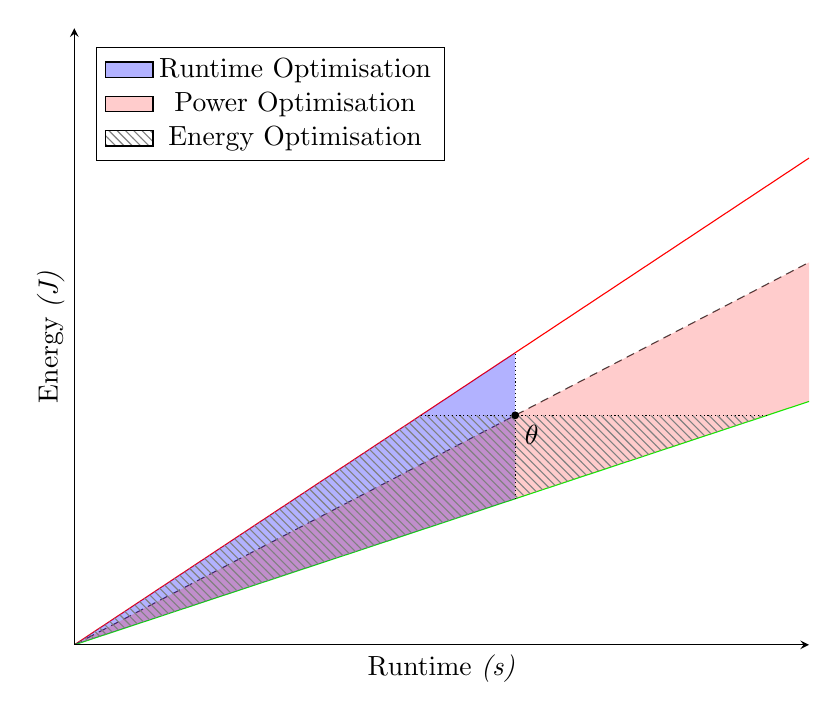
\begin{tikzpicture}
  \begin{axis}[ticks = none, 
    axis on top,
    axis x line=bottom,
    axis y line=left,
  	xlabel={Runtime \emph{(s)}},
    ylabel={Energy \emph{(J)}},    
    xmin=0, xmax=50,
    ymin=0, ymax=3800,
    width=0.9\linewidth,
    legend style={legend pos=north west}
    ]

    %% Model Parameters %%
    \pgfmathsetmacro{\baselinepower}{30} % NOP code
    \pgfmathsetmacro{\rooflinepower}{60}
    \pgfmathsetmacro{\codepower}{(\baselinepower*3 + \rooflinepower*4) / 7}
    \pgfmathsetmacro{\codetime}{30}
    % Sadly, pgfplots sucks too much to calculate cube roots
    \pgfmathsetmacro{\anodex}{26.20741}
    \pgfmathsetmacro{\anodey}{\anodex * \baselinepower}
    \pgfmathsetmacro{\cnodex}{34.34143}
    \pgfmathsetmacro{\cnodey}{\cnodex * \baselinepower}
    \pgfmathsetmacro{\tnodex}{27.25681}
 
    %% Intermezzo Values %%
    \pgfmathsetmacro{\codeenergy}{\codepower * \codetime}
    \pgfmathsetmacro{\baselineenergy}{\baselinepower * \codetime}
    \pgfmathsetmacro{\rooflineenergy}{\rooflinepower * \codetime}
    \pgfmathsetmacro{\lowdisplayline}{(2 * \baselinepower + \codepower) / 3}
    \pgfmathsetmacro{\highdisplayline}{(1 * \rooflinepower + 1 * \codepower) / 2}
    \pgfmathsetmacro{\rooflinetime}{\codeenergy/\rooflinepower}
    \pgfmathsetmacro{\baselinetime}{\codeenergy/\baselinepower}

    % arguments: code power, code time, x - todo, apparently not supposed to do pgfmathparse
    \pgfmathdeclarefunction{metricbound}{3}{%
      \pgfmathparse{((#1 * #2^3) / #3^2)}%
    }
    \pgfmathdeclarefunction{definitionbound}{3}{%
      \pgfmathparse{((#1 / #2^3) * #3^4)}%
    }
     \pgfmathdeclarefunction{optimisationlimits}{3}{%
      \pgfmathparse{(min(metricbound(#1, #2, #3), definitionbound(#1, #2, #3)))}
    }

    % BETA ROOFLINE BOUND
    \addplot[color=red, forget plot, domain=\pgfkeysvalueof{/pgfplots/xmin}:\pgfkeysvalueof{/pgfplots/xmax}] {\rooflinepower * x};

    %const power diagonal
    \addplot[color=darkgray, densely dashed, forget plot, %forget plot prevents legend entry
             domain=\pgfkeysvalueof{/pgfplots/xmin}:\pgfkeysvalueof{/pgfplots/xmax}] {\codepower * x}; 

    % ALPHA BASELINE BOUND 
    \addplot[color=green, forget plot, domain=\pgfkeysvalueof{/pgfplots/xmin}:\pgfkeysvalueof{/pgfplots/xmax}] {\baselinepower * x};

    %Runtime Optimisation
    \addplot[area legend, fill=blue, fill opacity=0.3, draw=none] coordinates { 
      (\codetime,\rooflineenergy)
      (\codetime,\baselineenergy)
    (0,0)};
    \addlegendentry{Runtime Optimisation}

    %Power Optimisation
    \addplot[area legend, fill=red, fill opacity=0.2, draw=none] coordinates {
                           (\codetime,\codeenergy)
                           (\pgfkeysvalueof{/pgfplots/xmax},\pgfkeysvalueof{/pgfplots/xmax}*\codepower)
                           (\pgfkeysvalueof{/pgfplots/xmax}, \pgfkeysvalueof{/pgfplots/xmax}*\baselinepower)
                           (0,0)
                         } ;
    \addlegendentry{Power Optimisation}
  
    %Energy Optimisation
    \addplot[area legend, style={pattern=north west lines, pattern color=gray,
                                 draw=none}] coordinates { 
      (\rooflinetime, \codeenergy)
      (\baselinetime, \codeenergy)
      (0, 0) };
    \addlegendentry{Energy Optimisation}



    % Constant Time, Energy Dashes
    %vertical
    \draw[densely dotted] ({axis cs:\codetime,\baselineenergy}) -- ({axis cs:\codetime,\rooflineenergy});
    %horizontal
    \draw[densely dotted] ({axis cs:\rooflinetime,\codeenergy}) -- ({axis cs:\baselinetime,\codeenergy});
   

    \node[circle,fill,inner sep=1pt] at (axis cs:\codetime,\codeenergy) {};
    \node[below right] at (axis cs:\codetime,\codeenergy) {$\theta$};


 \end{axis}
\end{tikzpicture}

    \end{figure}
  \end{frame}

  \begin{frame}
  \frametitle{Metrics}
  \begin{itemize}
  \item Our metric must combine both power and runtime
  \item Energy is a candidate in energy-critical domains
  \item Energy Delay Product (EDP) gives a greater weighting to runtime:
  \begin{align}
    EDP &= Energy \times Runtime \nonumber \\
        &= E \times t \nonumber \\
        &= \bar{P} \times t^2
  \end{align}
  \item $ED^2P$ and $ED^3P$ are also used.
  \item In general we refer to these as $E^mt^n$ metrics 
  \end{itemize}
  \end{frame}

  \begin{frame}
    \frametitle{Motivation for POSE}
    \begin{itemize}
      \item{How much a given code may benefit from energy optimisation}
      \begin{itemize}
        \item{Optimisation is expensive and time consuming}
        \item{Facilitates cost/benefit analysis}
      \end{itemize}
      \item{Whether to focus on reducing power or runtime}
      \begin{itemize}
        \item{A heuristic for sensitivity analysis}
        \item{Depends on the metric chosen}
      \end{itemize}
      \item{Whether an optimisation counts as energy optimisation}
      \begin{itemize}
        \item{Many purported energy optimisations simply reduce runtime}
      \end{itemize}
    \end{itemize}
   \end{frame}

  \begin{frame}
    \frametitle{Feasible Performance Envelope}
    \begin{itemize}
      \item POSE is built around the Feasible Performance Envelope
      \item The Feasible Performance Envelope contains all possible values for the rate of power consumption 
      \begin{itemize}
      \item Depicted as the area between lines of gradient $P_{max}$ and $P_{min}$
      \end{itemize}
      \item All $\langle Runtime, Energy \rangle$ program costs lie within this envelope
      \begin{itemize}
        \item For an initial code $\theta$, any modified version $\lambda$ must also exist within this envelope
      \end{itemize}
    \end{itemize}
  \end{frame}

  \begin{frame}
    \frametitle{Feasible Performance Envelope}
    \begin{figure}
    \centering
    \begin{tikzpicture}
  \begin{axis}[ticks = none, 
    axis on top,
    axis x line=bottom,
    axis y line=left,
  	xlabel={Runtime \emph{(s)}},
    ylabel={Energy \emph{(J)}},    
    xmin=0, xmax=50,
    ymin=0, ymax=3300,
    width=0.9\linewidth,
    legend style={legend pos=north west}
    ]

    %% Model Parameters %%
    \pgfmathsetmacro{\baselinepower}{30} % NOP code
    \pgfmathsetmacro{\rooflinepower}{60}
    \pgfmathsetmacro{\codepower}{47} 
    \pgfmathsetmacro{\codetime}{30}
    % Sadly, pgfplots sucks too much to calculate cube roots
    % These values are calculated with a ruby script in tools
    \pgfmathsetmacro{\blnodex}{25.83028}
    \pgfmathsetmacro{\brnodex}{34.84283}
    \pgfmathsetmacro{\trnodex}{27.65477}
    \pgfmathsetmacro{\tlnodex}{20.50151} % TODO

    %% Intermezzo Values %%
    \pgfmathsetmacro{\brnodey}{\brnodex * \baselinepower}
    \pgfmathsetmacro{\blnodey}{\blnodex * \baselinepower}
    \pgfmathsetmacro{\tlnodey}{\tlnodex * \rooflinepower}
    \pgfmathsetmacro{\trnodey}{\trnodex * \rooflinepower}
    \pgfmathsetmacro{\codeenergy}{\codepower * \codetime}
    \pgfmathsetmacro{\baselineenergy}{\baselinepower * \codetime}


    % arguments: code power, code time, x - todo, apparently not supposed to do pgfmathparse
    \pgfmathdeclarefunction{metricbound}{3}{%
      \pgfmathparse{((#1 * #2^3) / #3^2)}%
    }
    \pgfmathdeclarefunction{definitionbound}{3}{%
      \pgfmathparse{((#1 / #2^3) * #3^4)}%
    }

   % BETA ROOFLINE BOUND 
    \addplot[color=red, domain=\pgfkeysvalueof{/pgfplots/xmin}:\pgfkeysvalueof{/pgfplots/xmax}] {\rooflinepower * x};
    \addlegendentry{$P_{max}$ Energy Bound}

    % ALPHA BASELINE BOUND 
    \addplot[color=green, domain=\pgfkeysvalueof{/pgfplots/xmin}:\pgfkeysvalueof{/pgfplots/xmax}] {\baselinepower * x};
    \addlegendentry{$P_{min}$ Energy Bound} 



\ifdefined\OPTBOUND
    \addplot[color=orange, domain=\trnodex:\brnodex] { metricbound(\codepower, \codetime, x)};
    \addlegendentry{Optimisation Bound}
\fi

\ifdefined\CONTBOUND
    \addplot[color=blue!80, domain=\blnodex:\codetime] { definitionbound(\codepower, \codetime, x)};
    \addlegendentry{Contribution Bound}
\fi


\ifdefined\OPTLIMIT
    \addplot[color=orange, dashed, domain=\tlnodex:\blnodex] {metricbound(\baselinepower, \blnodex, x)};
    \addlegendentry{Optimisation Limit}
\fi

\ifdefined\POSELABELS
    % Constant Time (Vertical) dotted line
    \draw[densely dotted] ({axis cs:\codetime,\baselineenergy}) -- ({axis cs:\codetime,\codeenergy});


    \node [above left] at ({axis cs:\tlnodex, \tlnodey}) {A};
    \node [above left] at ({axis cs:\trnodex, \trnodey}) {B};
    \node [below right] at ({axis cs:\blnodex, \blnodey}) {C};
    \node [below right] at ({axis cs:\codetime,\baselineenergy}) {D};
    \node [below right=0cm] at ({axis cs:\brnodex, \brnodey}) {E};

    \pgfmathsetmacro{\onexcoord}{15}
    \node at (axis cs: \onexcoord, 44 * \onexcoord){1.};

    \pgfmathsetmacro{\twoxcoord}{25.8}
    \node at (axis cs: \twoxcoord, 44 * \twoxcoord){2.};

    \pgfmathsetmacro{\threexcoord}{\codetime+0.3}
    \node[fill=white] at (axis cs: \threexcoord, 36 * \codetime){3.};
    
    \pgfmathsetmacro{\fourxcoord}{40}
    \node at (axis cs: \fourxcoord, 44 * \fourxcoord){4.};

\fi

    \node[circle,fill,inner sep=1pt] at (axis cs:\codetime,\codeenergy) {};
    \node[above right] at (axis cs:\codetime,\codeenergy) {$\theta$};
 \end{axis}
\end{tikzpicture}

    \caption{Feasible Performance Envelope}
    \end{figure}
  \end{frame}

  \begin{frame}
    \frametitle{Measurement of $P_{max}$}
    \begin{itemize}
      \item Avoid vendor-published TDPs
      \begin{itemize}
        \item Typically Overly Conservative Estimates
      \end{itemize}
      \item Trialled several stress-test binaries
      \begin{itemize}
        \item Linpack
        \item Streams
        \item Prime95
        \item FIRESTARTER
      \end{itemize}
      \item Settled on FIRESTARTER as the most energy intensive
    \end{itemize}
  \end{frame}

  \begin{frame}
    \frametitle{Measurement of $P_{min}$}
    \begin{block}{$P_{min}$ Assembly Benchmark}
      \lstinputlisting[language=Python]{listings/noploop.asm}
    \end{block}
  \end{frame}




  \begin{frame}
    \frametitle{Optimisation Bound}
    \begin{definition}
    For two logically equivalent codes $\theta$ and $\lambda$, the transformation ${\theta \to \lambda}$ is a valid optimisation with respect to a cost metric $M$ if and only if ${M(\lambda) < M(\theta)}$. 
    \end{definition}
All optimized versions of $\theta$ must lie below the bound linking all points where ${M(\lambda) = M(\theta)}$.
\begin{align}
 {E_\lambda}^m{t_\lambda}^n &= {E_\theta}^m{t_\theta}^n \nonumber \\
 {E_\lambda}^m &= \frac{{E_\theta}^m{t_\theta}^n}{{t_\lambda}^n} \nonumber \\
  E_\lambda &= (\frac{{E_\theta}^m{t_\theta}^n}{{t_\lambda}^n})^\frac{1}{m}
\end{align}
  \end{frame}

  \begin{frame}
    \frametitle{$Et^2$ Optimisation Bound}
    \newcommand*{\OPTBOUND}{}%
    \begin{figure}
    \centering
    \begin{tikzpicture}
  \begin{axis}[ticks = none, 
    axis on top,
    axis x line=bottom,
    axis y line=left,
  	xlabel={Runtime \emph{(s)}},
    ylabel={Energy \emph{(J)}},    
    xmin=0, xmax=50,
    ymin=0, ymax=3300,
    width=0.9\linewidth,
    legend style={legend pos=north west}
    ]

    %% Model Parameters %%
    \pgfmathsetmacro{\baselinepower}{30} % NOP code
    \pgfmathsetmacro{\rooflinepower}{60}
    \pgfmathsetmacro{\codepower}{47} 
    \pgfmathsetmacro{\codetime}{30}
    % Sadly, pgfplots sucks too much to calculate cube roots
    % These values are calculated with a ruby script in tools
    \pgfmathsetmacro{\blnodex}{25.83028}
    \pgfmathsetmacro{\brnodex}{34.84283}
    \pgfmathsetmacro{\trnodex}{27.65477}
    \pgfmathsetmacro{\tlnodex}{20.50151} % TODO

    %% Intermezzo Values %%
    \pgfmathsetmacro{\brnodey}{\brnodex * \baselinepower}
    \pgfmathsetmacro{\blnodey}{\blnodex * \baselinepower}
    \pgfmathsetmacro{\tlnodey}{\tlnodex * \rooflinepower}
    \pgfmathsetmacro{\trnodey}{\trnodex * \rooflinepower}
    \pgfmathsetmacro{\codeenergy}{\codepower * \codetime}
    \pgfmathsetmacro{\baselineenergy}{\baselinepower * \codetime}


    % arguments: code power, code time, x - todo, apparently not supposed to do pgfmathparse
    \pgfmathdeclarefunction{metricbound}{3}{%
      \pgfmathparse{((#1 * #2^3) / #3^2)}%
    }
    \pgfmathdeclarefunction{definitionbound}{3}{%
      \pgfmathparse{((#1 / #2^3) * #3^4)}%
    }

   % BETA ROOFLINE BOUND 
    \addplot[color=red, domain=\pgfkeysvalueof{/pgfplots/xmin}:\pgfkeysvalueof{/pgfplots/xmax}] {\rooflinepower * x};
    \addlegendentry{$P_{max}$ Energy Bound}

    % ALPHA BASELINE BOUND 
    \addplot[color=green, domain=\pgfkeysvalueof{/pgfplots/xmin}:\pgfkeysvalueof{/pgfplots/xmax}] {\baselinepower * x};
    \addlegendentry{$P_{min}$ Energy Bound} 



\ifdefined\OPTBOUND
    \addplot[color=orange, domain=\trnodex:\brnodex] { metricbound(\codepower, \codetime, x)};
    \addlegendentry{Optimisation Bound}
\fi

\ifdefined\CONTBOUND
    \addplot[color=blue!80, domain=\blnodex:\codetime] { definitionbound(\codepower, \codetime, x)};
    \addlegendentry{Contribution Bound}
\fi


\ifdefined\OPTLIMIT
    \addplot[color=orange, dashed, domain=\tlnodex:\blnodex] {metricbound(\baselinepower, \blnodex, x)};
    \addlegendentry{Optimisation Limit}
\fi

\ifdefined\POSELABELS
    % Constant Time (Vertical) dotted line
    \draw[densely dotted] ({axis cs:\codetime,\baselineenergy}) -- ({axis cs:\codetime,\codeenergy});


    \node [above left] at ({axis cs:\tlnodex, \tlnodey}) {A};
    \node [above left] at ({axis cs:\trnodex, \trnodey}) {B};
    \node [below right] at ({axis cs:\blnodex, \blnodey}) {C};
    \node [below right] at ({axis cs:\codetime,\baselineenergy}) {D};
    \node [below right=0cm] at ({axis cs:\brnodex, \brnodey}) {E};

    \pgfmathsetmacro{\onexcoord}{15}
    \node at (axis cs: \onexcoord, 44 * \onexcoord){1.};

    \pgfmathsetmacro{\twoxcoord}{25.8}
    \node at (axis cs: \twoxcoord, 44 * \twoxcoord){2.};

    \pgfmathsetmacro{\threexcoord}{\codetime+0.3}
    \node[fill=white] at (axis cs: \threexcoord, 36 * \codetime){3.};
    
    \pgfmathsetmacro{\fourxcoord}{40}
    \node at (axis cs: \fourxcoord, 44 * \fourxcoord){4.};

\fi

    \node[circle,fill,inner sep=1pt] at (axis cs:\codetime,\codeenergy) {};
    \node[above right] at (axis cs:\codetime,\codeenergy) {$\theta$};
 \end{axis}
\end{tikzpicture}

    \end{figure}
  \end{frame}

  \begin{frame}
    \frametitle{Contribution Bound}
    \begin{definition}
      Optimisation $\theta \to \lambda$ with respect to metric $M$ to be a power optimisation if the change in power draw it delivers is responsible for the majority of the reduction in $M$. 
      \end{definition}
 All power-optimised versions of $\theta$ must lie below the bound linking all points for which power and runtime factors contribute to $M$ in the same ratio as $\theta$.
\begin{align}
\frac{{P_{\lambda}}^m}{{t_{\lambda}}^{m+n}} &= \frac{{P_{\theta}}^m}{{t_{\theta}}^{m+n}} \nonumber \\
 {P_{\lambda}}^m &= \frac{{P_{\theta}}^m}{{t_{\theta}}^{m+n}} \times {t_\lambda}^{m+n} \nonumber \\ 
 {E_{\lambda}}^m &= \frac{{P_{\theta}}^m}{{t_{\theta}}^{m+n}} \times {t_\lambda}^{m+n+1} \nonumber \\ 
  E_{\lambda} &= (\frac{{P_{\theta}}^m}{{t_{\theta}}^{m+n}} \times {t_\lambda}^{m+n+1})^{\frac{1}{m}} 
\end{align}
  \end{frame}

  \begin{frame}
    \frametitle{$Et^2$ Contribution Bound}
    \newcommand*{\OPTBOUND}{}%
    \newcommand*{\CONTBOUND}{}%
    \begin{figure}
    \centering
    \begin{tikzpicture}
  \begin{axis}[ticks = none, 
    axis on top,
    axis x line=bottom,
    axis y line=left,
  	xlabel={Runtime \emph{(s)}},
    ylabel={Energy \emph{(J)}},    
    xmin=0, xmax=50,
    ymin=0, ymax=3300,
    width=0.9\linewidth,
    legend style={legend pos=north west}
    ]

    %% Model Parameters %%
    \pgfmathsetmacro{\baselinepower}{30} % NOP code
    \pgfmathsetmacro{\rooflinepower}{60}
    \pgfmathsetmacro{\codepower}{47} 
    \pgfmathsetmacro{\codetime}{30}
    % Sadly, pgfplots sucks too much to calculate cube roots
    % These values are calculated with a ruby script in tools
    \pgfmathsetmacro{\blnodex}{25.83028}
    \pgfmathsetmacro{\brnodex}{34.84283}
    \pgfmathsetmacro{\trnodex}{27.65477}
    \pgfmathsetmacro{\tlnodex}{20.50151} % TODO

    %% Intermezzo Values %%
    \pgfmathsetmacro{\brnodey}{\brnodex * \baselinepower}
    \pgfmathsetmacro{\blnodey}{\blnodex * \baselinepower}
    \pgfmathsetmacro{\tlnodey}{\tlnodex * \rooflinepower}
    \pgfmathsetmacro{\trnodey}{\trnodex * \rooflinepower}
    \pgfmathsetmacro{\codeenergy}{\codepower * \codetime}
    \pgfmathsetmacro{\baselineenergy}{\baselinepower * \codetime}


    % arguments: code power, code time, x - todo, apparently not supposed to do pgfmathparse
    \pgfmathdeclarefunction{metricbound}{3}{%
      \pgfmathparse{((#1 * #2^3) / #3^2)}%
    }
    \pgfmathdeclarefunction{definitionbound}{3}{%
      \pgfmathparse{((#1 / #2^3) * #3^4)}%
    }

   % BETA ROOFLINE BOUND 
    \addplot[color=red, domain=\pgfkeysvalueof{/pgfplots/xmin}:\pgfkeysvalueof{/pgfplots/xmax}] {\rooflinepower * x};
    \addlegendentry{$P_{max}$ Energy Bound}

    % ALPHA BASELINE BOUND 
    \addplot[color=green, domain=\pgfkeysvalueof{/pgfplots/xmin}:\pgfkeysvalueof{/pgfplots/xmax}] {\baselinepower * x};
    \addlegendentry{$P_{min}$ Energy Bound} 



\ifdefined\OPTBOUND
    \addplot[color=orange, domain=\trnodex:\brnodex] { metricbound(\codepower, \codetime, x)};
    \addlegendentry{Optimisation Bound}
\fi

\ifdefined\CONTBOUND
    \addplot[color=blue!80, domain=\blnodex:\codetime] { definitionbound(\codepower, \codetime, x)};
    \addlegendentry{Contribution Bound}
\fi


\ifdefined\OPTLIMIT
    \addplot[color=orange, dashed, domain=\tlnodex:\blnodex] {metricbound(\baselinepower, \blnodex, x)};
    \addlegendentry{Optimisation Limit}
\fi

\ifdefined\POSELABELS
    % Constant Time (Vertical) dotted line
    \draw[densely dotted] ({axis cs:\codetime,\baselineenergy}) -- ({axis cs:\codetime,\codeenergy});


    \node [above left] at ({axis cs:\tlnodex, \tlnodey}) {A};
    \node [above left] at ({axis cs:\trnodex, \trnodey}) {B};
    \node [below right] at ({axis cs:\blnodex, \blnodey}) {C};
    \node [below right] at ({axis cs:\codetime,\baselineenergy}) {D};
    \node [below right=0cm] at ({axis cs:\brnodex, \brnodey}) {E};

    \pgfmathsetmacro{\onexcoord}{15}
    \node at (axis cs: \onexcoord, 44 * \onexcoord){1.};

    \pgfmathsetmacro{\twoxcoord}{25.8}
    \node at (axis cs: \twoxcoord, 44 * \twoxcoord){2.};

    \pgfmathsetmacro{\threexcoord}{\codetime+0.3}
    \node[fill=white] at (axis cs: \threexcoord, 36 * \codetime){3.};
    
    \pgfmathsetmacro{\fourxcoord}{40}
    \node at (axis cs: \fourxcoord, 44 * \fourxcoord){4.};

\fi

    \node[circle,fill,inner sep=1pt] at (axis cs:\codetime,\codeenergy) {};
    \node[above right] at (axis cs:\codetime,\codeenergy) {$\theta$};
 \end{axis}
\end{tikzpicture}

    \end{figure}
  \end{frame}


  \begin{frame}
    \frametitle{Optimisation Limit}
    \begin{itemize}
      \item Shares same definition as Optimisation Bound, except drawn from the maximally power optimised point
      \item Subdivides runtime optimized area of the Feasible Performance Area
      \begin{itemize}
        \item Optimisations dominated by best possible power optimisation
        \item Optimisations which dominate best possible power optimisation
      \end{itemize}
    \end{itemize}
  \end{frame}

  \begin{frame}
    \frametitle{$Et^2$ Optimisation Limit}
    \newcommand*{\OPTBOUND}{}%
    \newcommand*{\CONTBOUND}{}% 
    \newcommand*{\OPTLIMIT}{}%
    \begin{figure}
    \centering
    \begin{tikzpicture}
  \begin{axis}[ticks = none, 
    axis on top,
    axis x line=bottom,
    axis y line=left,
  	xlabel={Runtime \emph{(s)}},
    ylabel={Energy \emph{(J)}},    
    xmin=0, xmax=50,
    ymin=0, ymax=3300,
    width=0.9\linewidth,
    legend style={legend pos=north west}
    ]

    %% Model Parameters %%
    \pgfmathsetmacro{\baselinepower}{30} % NOP code
    \pgfmathsetmacro{\rooflinepower}{60}
    \pgfmathsetmacro{\codepower}{47} 
    \pgfmathsetmacro{\codetime}{30}
    % Sadly, pgfplots sucks too much to calculate cube roots
    % These values are calculated with a ruby script in tools
    \pgfmathsetmacro{\blnodex}{25.83028}
    \pgfmathsetmacro{\brnodex}{34.84283}
    \pgfmathsetmacro{\trnodex}{27.65477}
    \pgfmathsetmacro{\tlnodex}{20.50151} % TODO

    %% Intermezzo Values %%
    \pgfmathsetmacro{\brnodey}{\brnodex * \baselinepower}
    \pgfmathsetmacro{\blnodey}{\blnodex * \baselinepower}
    \pgfmathsetmacro{\tlnodey}{\tlnodex * \rooflinepower}
    \pgfmathsetmacro{\trnodey}{\trnodex * \rooflinepower}
    \pgfmathsetmacro{\codeenergy}{\codepower * \codetime}
    \pgfmathsetmacro{\baselineenergy}{\baselinepower * \codetime}


    % arguments: code power, code time, x - todo, apparently not supposed to do pgfmathparse
    \pgfmathdeclarefunction{metricbound}{3}{%
      \pgfmathparse{((#1 * #2^3) / #3^2)}%
    }
    \pgfmathdeclarefunction{definitionbound}{3}{%
      \pgfmathparse{((#1 / #2^3) * #3^4)}%
    }

   % BETA ROOFLINE BOUND 
    \addplot[color=red, domain=\pgfkeysvalueof{/pgfplots/xmin}:\pgfkeysvalueof{/pgfplots/xmax}] {\rooflinepower * x};
    \addlegendentry{$P_{max}$ Energy Bound}

    % ALPHA BASELINE BOUND 
    \addplot[color=green, domain=\pgfkeysvalueof{/pgfplots/xmin}:\pgfkeysvalueof{/pgfplots/xmax}] {\baselinepower * x};
    \addlegendentry{$P_{min}$ Energy Bound} 



\ifdefined\OPTBOUND
    \addplot[color=orange, domain=\trnodex:\brnodex] { metricbound(\codepower, \codetime, x)};
    \addlegendentry{Optimisation Bound}
\fi

\ifdefined\CONTBOUND
    \addplot[color=blue!80, domain=\blnodex:\codetime] { definitionbound(\codepower, \codetime, x)};
    \addlegendentry{Contribution Bound}
\fi


\ifdefined\OPTLIMIT
    \addplot[color=orange, dashed, domain=\tlnodex:\blnodex] {metricbound(\baselinepower, \blnodex, x)};
    \addlegendentry{Optimisation Limit}
\fi

\ifdefined\POSELABELS
    % Constant Time (Vertical) dotted line
    \draw[densely dotted] ({axis cs:\codetime,\baselineenergy}) -- ({axis cs:\codetime,\codeenergy});


    \node [above left] at ({axis cs:\tlnodex, \tlnodey}) {A};
    \node [above left] at ({axis cs:\trnodex, \trnodey}) {B};
    \node [below right] at ({axis cs:\blnodex, \blnodey}) {C};
    \node [below right] at ({axis cs:\codetime,\baselineenergy}) {D};
    \node [below right=0cm] at ({axis cs:\brnodex, \brnodey}) {E};

    \pgfmathsetmacro{\onexcoord}{15}
    \node at (axis cs: \onexcoord, 44 * \onexcoord){1.};

    \pgfmathsetmacro{\twoxcoord}{25.8}
    \node at (axis cs: \twoxcoord, 44 * \twoxcoord){2.};

    \pgfmathsetmacro{\threexcoord}{\codetime+0.3}
    \node[fill=white] at (axis cs: \threexcoord, 36 * \codetime){3.};
    
    \pgfmathsetmacro{\fourxcoord}{40}
    \node at (axis cs: \fourxcoord, 44 * \fourxcoord){4.};

\fi

    \node[circle,fill,inner sep=1pt] at (axis cs:\codetime,\codeenergy) {};
    \node[above right] at (axis cs:\codetime,\codeenergy) {$\theta$};
 \end{axis}
\end{tikzpicture}

    \end{figure}
  \end{frame}

  \begin{frame}
    \frametitle{$Et^2$ POSE}
    \newcommand*{\OPTBOUND}{}%
    \newcommand*{\CONTBOUND}{}% 
    \newcommand*{\OPTLIMIT}{}%
    \newcommand*{\POSELABELS}{}%
    \begin{figure}
    \centering
    \begin{tikzpicture}
  \begin{axis}[ticks = none, 
    axis on top,
    axis x line=bottom,
    axis y line=left,
  	xlabel={Runtime \emph{(s)}},
    ylabel={Energy \emph{(J)}},    
    xmin=0, xmax=50,
    ymin=0, ymax=3300,
    width=0.9\linewidth,
    legend style={legend pos=north west}
    ]

    %% Model Parameters %%
    \pgfmathsetmacro{\baselinepower}{30} % NOP code
    \pgfmathsetmacro{\rooflinepower}{60}
    \pgfmathsetmacro{\codepower}{47} 
    \pgfmathsetmacro{\codetime}{30}
    % Sadly, pgfplots sucks too much to calculate cube roots
    % These values are calculated with a ruby script in tools
    \pgfmathsetmacro{\blnodex}{25.83028}
    \pgfmathsetmacro{\brnodex}{34.84283}
    \pgfmathsetmacro{\trnodex}{27.65477}
    \pgfmathsetmacro{\tlnodex}{20.50151} % TODO

    %% Intermezzo Values %%
    \pgfmathsetmacro{\brnodey}{\brnodex * \baselinepower}
    \pgfmathsetmacro{\blnodey}{\blnodex * \baselinepower}
    \pgfmathsetmacro{\tlnodey}{\tlnodex * \rooflinepower}
    \pgfmathsetmacro{\trnodey}{\trnodex * \rooflinepower}
    \pgfmathsetmacro{\codeenergy}{\codepower * \codetime}
    \pgfmathsetmacro{\baselineenergy}{\baselinepower * \codetime}


    % arguments: code power, code time, x - todo, apparently not supposed to do pgfmathparse
    \pgfmathdeclarefunction{metricbound}{3}{%
      \pgfmathparse{((#1 * #2^3) / #3^2)}%
    }
    \pgfmathdeclarefunction{definitionbound}{3}{%
      \pgfmathparse{((#1 / #2^3) * #3^4)}%
    }

   % BETA ROOFLINE BOUND 
    \addplot[color=red, domain=\pgfkeysvalueof{/pgfplots/xmin}:\pgfkeysvalueof{/pgfplots/xmax}] {\rooflinepower * x};
    \addlegendentry{$P_{max}$ Energy Bound}

    % ALPHA BASELINE BOUND 
    \addplot[color=green, domain=\pgfkeysvalueof{/pgfplots/xmin}:\pgfkeysvalueof{/pgfplots/xmax}] {\baselinepower * x};
    \addlegendentry{$P_{min}$ Energy Bound} 



\ifdefined\OPTBOUND
    \addplot[color=orange, domain=\trnodex:\brnodex] { metricbound(\codepower, \codetime, x)};
    \addlegendentry{Optimisation Bound}
\fi

\ifdefined\CONTBOUND
    \addplot[color=blue!80, domain=\blnodex:\codetime] { definitionbound(\codepower, \codetime, x)};
    \addlegendentry{Contribution Bound}
\fi


\ifdefined\OPTLIMIT
    \addplot[color=orange, dashed, domain=\tlnodex:\blnodex] {metricbound(\baselinepower, \blnodex, x)};
    \addlegendentry{Optimisation Limit}
\fi

\ifdefined\POSELABELS
    % Constant Time (Vertical) dotted line
    \draw[densely dotted] ({axis cs:\codetime,\baselineenergy}) -- ({axis cs:\codetime,\codeenergy});


    \node [above left] at ({axis cs:\tlnodex, \tlnodey}) {A};
    \node [above left] at ({axis cs:\trnodex, \trnodey}) {B};
    \node [below right] at ({axis cs:\blnodex, \blnodey}) {C};
    \node [below right] at ({axis cs:\codetime,\baselineenergy}) {D};
    \node [below right=0cm] at ({axis cs:\brnodex, \brnodey}) {E};

    \pgfmathsetmacro{\onexcoord}{15}
    \node at (axis cs: \onexcoord, 44 * \onexcoord){1.};

    \pgfmathsetmacro{\twoxcoord}{25.8}
    \node at (axis cs: \twoxcoord, 44 * \twoxcoord){2.};

    \pgfmathsetmacro{\threexcoord}{\codetime+0.3}
    \node[fill=white] at (axis cs: \threexcoord, 36 * \codetime){3.};
    
    \pgfmathsetmacro{\fourxcoord}{40}
    \node at (axis cs: \fourxcoord, 44 * \fourxcoord){4.};

\fi

    \node[circle,fill,inner sep=1pt] at (axis cs:\codetime,\codeenergy) {};
    \node[above right] at (axis cs:\codetime,\codeenergy) {$\theta$};
 \end{axis}
\end{tikzpicture}

    \end{figure}
  \end{frame}




  \begin{frame}
    \frametitle{Metric Agnostic POSE}
    \begin{figure}
    \centering
    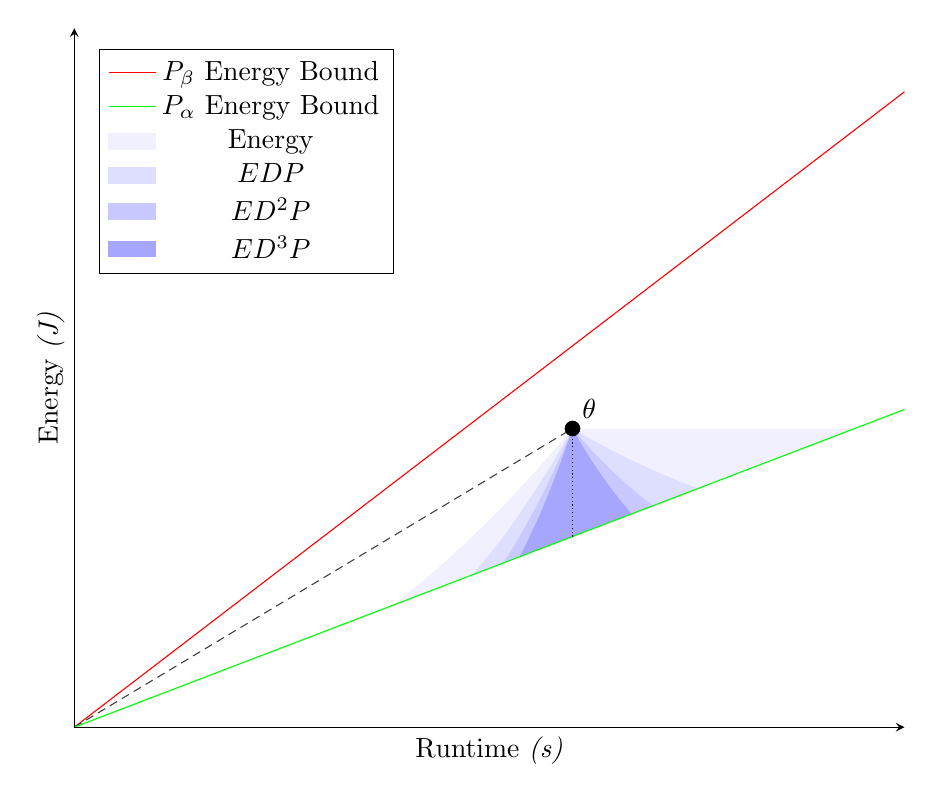
\begin{tikzpicture}
  \begin{axis}[ticks = none, 
    axis on top,
    axis x line=bottom,
    axis y line=left,
  	xlabel={Runtime \emph{(s)}},
    ylabel={Energy \emph{(J)}},    
    xmin=0, xmax=50,
    ymin=0, ymax=3300,
    width=\linewidth,
    legend style={legend pos=north west}
    ]

    %% Model Parameters %%
    \pgfmathsetmacro{\baselinepower}{30} % NOP code
    \pgfmathsetmacro{\rooflinepower}{60}
    \pgfmathsetmacro{\codepower}{47} 
    \pgfmathsetmacro{\codetime}{30}




    %% Intermezzo Values %%
    \pgfmathsetmacro{\codeenergy}{\codepower * \codetime}
    \pgfmathsetmacro{\baselineenergy}{\baselinepower * \codetime}
    \pgfmathsetmacro{\rooflineenergy}{\rooflinepower * \codetime}
    \pgfmathsetmacro{\lowdisplayline}{(2 * \baselinepower + \codepower) / 3}
    \pgfmathsetmacro{\highdisplayline}{(1 * \rooflinepower + 1 * \codepower) / 2}

    % arguments: code power, code time, x, n 
    \pgfmathdeclarefunction{metricbound}{4}{%
      \pgfmathparse{((#1 * #2^(#4 + 1)) / #3^#4)}%
    }
    \pgfmathdeclarefunction{definitionbound}{4}{%
      \pgfmathparse{((#1 / #2^(#4 + 1)) * #3^(#4 + 2))}%
    }
 
    % BETA ROOFLINE BOUND
    \addplot[color=red, domain=\pgfkeysvalueof{/pgfplots/xmin}:\pgfkeysvalueof{/pgfplots/xmax}] {\rooflinepower * x};
    \addlegendentry{$P_{\beta}$ Energy Bound}

    %const power diagonal
    \addplot[color=darkgray, densely dashed, name path=constpwr, forget plot, %forget plot prevents legend entry
            domain=\pgfkeysvalueof{/pgfplots/xmin}:\codetime] {\codepower * x}; 

    % ALPHA BASELINE BOUND 
    \addplot[color=green, name path=basebound, domain=\pgfkeysvalueof{/pgfplots/xmin}:\pgfkeysvalueof{/pgfplots/xmax}] {\baselinepower * x};
    \addlegendentry{$P_{\alpha}$ Energy Bound} 

    % Constant Time vertical dots
    %vertical
    \draw[densely dotted] ({axis cs:\codetime,\baselineenergy}) -- ({axis cs:\codetime,\codeenergy});

    % Sadly, pgfplots sucks too much to calculate cube roots
    % Domain values are calculated with a ruby script in tools

    %% Energy Area %%
    \addplot[name path=energy, draw=none, domain=19.14894:47, forget plot]{ min(definitionbound(\codepower, \codetime, x, 0),metricbound(\codepower, \codetime, x, 0))};
    \addplot[blue!6] fill between[of=energy and basebound];
    \addlegendentry{Energy}

    %% Energy Delay Product Area %% 
    \addplot[name path=edp, draw=none, domain=23.96806:37.54997, forget plot] { min(definitionbound(\codepower, \codetime, x, 1),metricbound(\codepower, \codetime, x, 1))};
    \addplot[blue!13] fill between[of=edp and basebound];
    \addlegendentry{$EDP$}

    %% Energy Delay Squared Product Area ##
    \addplot[name path=edtwop, draw=none, domain=25.83028:34.84283, forget plot] { min(definitionbound(\codepower, \codetime, x, 2),metricbound(\codepower, \codetime, x, 2))};
    \addplot[blue!21] fill between[of=edtwop and basebound];
    \addlegendentry{$ED^2P$}

    %% Energy Delay Cubed Product Area ##
    \addplot[name path=edthreep, draw=none, domain=26.81496:33.56336, forget plot] { min(definitionbound(\codepower, \codetime, x, 3),metricbound(\codepower, \codetime, x, 3))};
    \addplot[blue!35] fill between[of=edthreep and basebound];
    \addlegendentry{$ED^3P$}




     \node[circle,fill,inner sep=2pt] at (axis cs:\codetime,\codeenergy) {};
    \node[above right] at (axis cs:\codetime,\codeenergy) {$\theta$};
  \end{axis}
\end{tikzpicture}

    \end{figure}
  \end{frame}






  \begin{frame}
    \frametitle{Investigation}
    \begin{itemize}
      \item CPU power consumption of Molecular Dynamics miniapps
      \begin{itemize}
        \item MiniMD
        \item LavaMD
      \end{itemize}
      \item Intel RAPL for power measurements
    \end{itemize}
  \end{frame}



  \begin{frame}
    \frametitle{MiniMD}
    \begin{figure}
    \providecommand{\plotwidth}{.8\linewidth}
    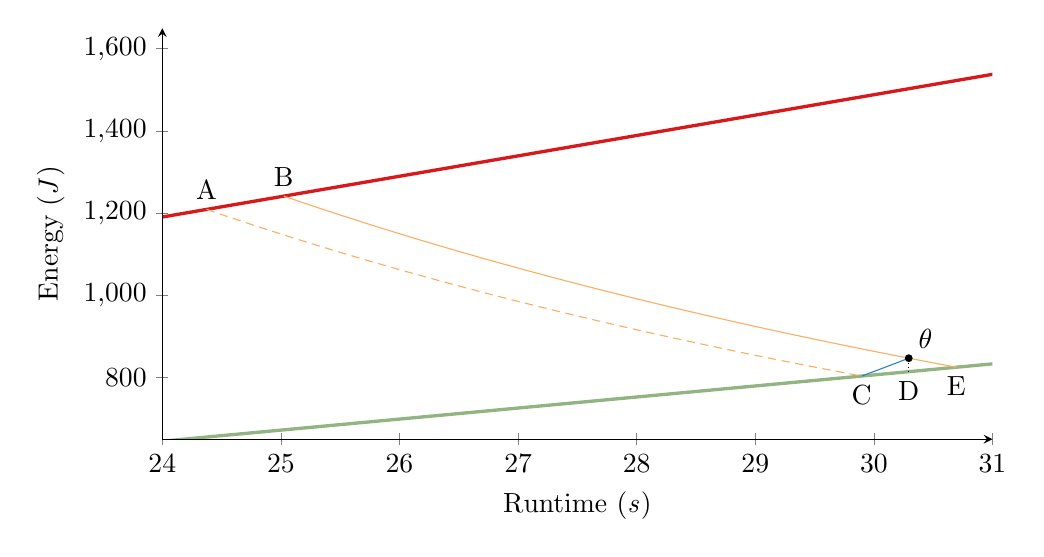
\begin{tikzpicture}
  \providecommand{\plotwidth}{\linewidth}
  \begin{axis}[
    axis on top,
    axis x line=bottom,
    axis y line=left,
    xlabel={Runtime (\emph{s})},
    ylabel={Energy (\emph{J})},    
    xmin=24, xmax=31,
    ymin=650, ymax=1650,
    width=\plotwidth,
    height=6.8cm,
    legend columns=3,
    legend to name=minimd:legend,
    legend style={/tikz/every even column/.append style={column sep=0.2cm}} % space out columns a bit
    ]

    %% Model Parameters %%
    \pgfmathsetmacro{\baselinepower}{26.876067}
    \pgfmathsetmacro{\rooflinepower}{49.60612}
    \pgfmathsetmacro{\codepower}{27.95947000000066} 
    \pgfmathsetmacro{\codetime}{30.293834}
    \pgfmathsetmacro{\codeenergy}{846.999542908}
    \pgfmathsetmacro{\energyexp}{1.0}
    \pgfmathsetmacro{\timeexp}{2.0}

    % Sadly, pgfplots sucks too much to calculate cube roots
    % These values are calculated with a ruby script in tools
    \pgfmathsetmacro{\blnodex}{29.897382525363728}
    \pgfmathsetmacro{\brnodex}{30.69554258273286}
    \pgfmathsetmacro{\trnodex}{25.0237350439618}
    \pgfmathsetmacro{\tlnodex}{24.373056016397907}

    %% Intermezzo Values %%
    \pgfmathsetmacro{\brnodey}{\brnodex * \baselinepower}
    \pgfmathsetmacro{\blnodey}{\blnodex * \baselinepower}
    \pgfmathsetmacro{\tlnodey}{\tlnodex * \rooflinepower}
    \pgfmathsetmacro{\trnodey}{\trnodex * \rooflinepower}
    \pgfmathsetmacro{\codeenergy}{\codepower * \codetime}
    \pgfmathsetmacro{\baselineenergy}{\baselinepower * \codetime}

    % arguments: code power, code time, x - todo, apparently not supposed to do pgfmathparse
    \pgfmathdeclarefunction{metricbound}{3}{%
      \pgfmathparse{((#1 * #2^3) / #3^2)}%
    }
    \pgfmathdeclarefunction{definitionbound}{3}{%
      \pgfmathparse{((#1 / #2^3) * #3^4)}%
    }

   % BETA ROOFLINE BOUND 
    \addplot[color=printred, very thick, domain=\pgfkeysvalueof{/pgfplots/xmin}:\pgfkeysvalueof{/pgfplots/xmax}] {\rooflinepower * x};
    \addlegendentry{$P_{max}$ Energy Bound}

    % ALPHA BASELINE BOUND 
    \addplot[color=printgreen, very thick, domain=\pgfkeysvalueof{/pgfplots/xmin}:\pgfkeysvalueof{/pgfplots/xmax}] {\baselinepower * x};
    \addlegendentry{$P_{min}$ Energy Bound} 

    \addplot[color=printorange, domain=\trnodex:\brnodex] { metricbound(\codepower, \codetime, x)};
    \addlegendentry{Optimisation Bound}

    \addplot[color=printblue, domain=\blnodex:\codetime] { definitionbound(\codepower, \codetime, x)};
    \addlegendentry{Contribution Bound}

    \addplot[color=printorange, densely dashed, domain=\tlnodex:\blnodex] {metricbound(\baselinepower, \blnodex, x)};
    \addlegendentry{Optimisation Limit}

    % Constant Time (Vertical) dotted line
    \draw[densely dotted] ({axis cs:\codetime,\baselineenergy}) -- ({axis cs:\codetime,\codeenergy});

    \node[circle,fill,inner sep=1pt] at (axis cs:\codetime,\codeenergy) {};
    \node[above right] at (axis cs:\codetime,\codeenergy) {$\theta$};
    
    \node [above] at ({axis cs:\tlnodex, \tlnodey}) {A};
    \node [above] at ({axis cs:\trnodex, \trnodey}) {B};
    \node [below] at ({axis cs:\blnodex, \blnodey}) {C};
    \node [below] at ({axis cs:\codetime,\baselineenergy}) {D};
    \node [below] at ({axis cs:\brnodex, \brnodey}) {E};
 \end{axis}
\end{tikzpicture}

    \end{figure}
  \end{frame}
  \begin{frame}
    \frametitle{MiniMD}
    \begin{table}
    \input{tab/tex/minimd_pose}
    \caption{MiniMD POSE, 4 cores 3.2GHz}
    \end{table} 
  \end{frame}

  \begin{frame}
    \frametitle{MiniMD Report}
    For MiniMD, the longest runtime within the Power Optimized Software Envelope is 30.70s.
    This means that any optimization which trades increased runtime for improved power efficiency can slow MiniMD down by at most 0.41s before $Et^2$ becomes strictly worse.
    The upper limit of energy to be saved from power optimisation alone for MiniMD running on our target platform is is 32.82J.

    The lowest value of $Et^2$ within the envelope is 718232.78, an improvement of 7.60\% over the baseline code. 
    Runtime optimization will be required to deliver any improvements above this level.
    We also know that a speedup of, 1.16x, or 4.16s, is guaranteed to beat $\theta$ in terms of $Et^2$.
    Finally, a speedup of 1.19x, or 4.84s, is guaranteed to beat any power optimised version of $\theta$ in terms of $Et^2$
  \end{frame}

  \begin{frame}
    \frametitle{LavaMD}
    \begin{figure}
    \providecommand{\plotwidth}{.8\linewidth}
    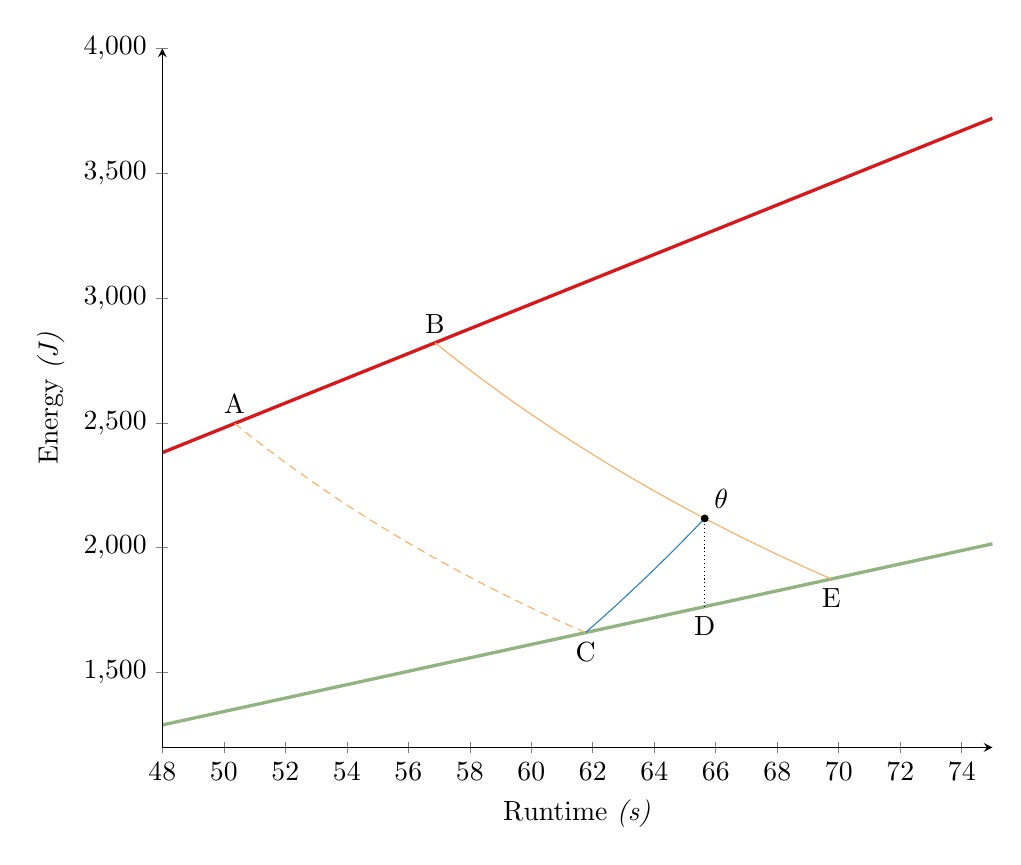
\begin{tikzpicture}
  \providecommand{\plotwidth}{\linewidth}
  \begin{axis}[
    axis on top,
    axis x line=bottom,
    axis y line=left,
  	xlabel={Runtime \emph{(s)}},
    ylabel={Energy \emph{(J)}},    
    xmin=48, xmax=75,
    ymin=1200, ymax=4000,
    width=\plotwidth,
    legend to name=lavamd:legend
    ]


    %% Model Parameters %%
    \pgfmathsetmacro{\baselinepower}{26.876067}
    \pgfmathsetmacro{\rooflinepower}{49.60612}
    \pgfmathsetmacro{\codepower}{32.25937199992712} 
    \pgfmathsetmacro{\codetime}{65.640072}
    \pgfmathsetmacro{\codeenergy}{2117.50750075}
    \pgfmathsetmacro{\energyexp}{1.0}
    \pgfmathsetmacro{\timeexp}{2.0}

    % Sadly, pgfplots sucks too much to calculate cube roots
    % These values are calculated with a ruby script in tools
    \pgfmathsetmacro{\blnodex}{61.76450770785698}
    \pgfmathsetmacro{\brnodex}{69.75881800183261}
    \pgfmathsetmacro{\trnodex}{56.869044551106185}
    \pgfmathsetmacro{\tlnodex}{50.35189300975517}
   
    %% Intermezzo Values %%
    \pgfmathsetmacro{\brnodey}{\brnodex * \baselinepower}
    \pgfmathsetmacro{\blnodey}{\blnodex * \baselinepower}
    \pgfmathsetmacro{\tlnodey}{\tlnodex * \rooflinepower}
    \pgfmathsetmacro{\trnodey}{\trnodex * \rooflinepower}
    \pgfmathsetmacro{\codeenergy}{\codepower * \codetime}
    \pgfmathsetmacro{\baselineenergy}{\baselinepower * \codetime}

    % arguments: code power, code time, x - todo, apparently not supposed to do pgfmathparse
    \pgfmathdeclarefunction{metricbound}{3}{%
      \pgfmathparse{((#1 * #2^3) / #3^2)}%
    }
    \pgfmathdeclarefunction{definitionbound}{3}{%
      \pgfmathparse{((#1 / #2^3) * #3^4)}%
    }


   % BETA ROOFLINE BOUND 
    \addplot[color=printred, very thick, domain=\pgfkeysvalueof{/pgfplots/xmin}:\pgfkeysvalueof{/pgfplots/xmax}] {\rooflinepower * x};
    \addlegendentry{$P_{max}$ Energy Bound}

    % ALPHA BASELINE BOUND 
    \addplot[color=printgreen, very thick, domain=\pgfkeysvalueof{/pgfplots/xmin}:\pgfkeysvalueof{/pgfplots/xmax}] {\baselinepower * x};
    \addlegendentry{$P_{min}$ Energy Bound} 

    \addplot[color=printorange, domain=\trnodex:\brnodex] { metricbound(\codepower, \codetime, x)};
    \addlegendentry{Optimisation Bound}

    \addplot[color=printblue, domain=\blnodex:\codetime] { definitionbound(\codepower, \codetime, x)};
    \addlegendentry{Contribution Bound}

    \addplot[color=printorange, densely dashed, domain=\tlnodex:\blnodex] {metricbound(\baselinepower, \blnodex, x)};
    \addlegendentry{Optimisation Limit}

    % Constant Time (Vertical) dotted line
    \draw[densely dotted] ({axis cs:\codetime,\baselineenergy}) -- ({axis cs:\codetime,\codeenergy});

    \node[circle,fill,inner sep=1pt] at (axis cs:\codetime,\codeenergy) {};
    \node[above right] at (axis cs:\codetime,\codeenergy) {$\theta$};
    
    \node [above] at ({axis cs:\tlnodex, \tlnodey}) {A};
    \node [above] at ({axis cs:\trnodex, \trnodey}) {B};
    \node [below] at ({axis cs:\blnodex, \blnodey}) {C};
    \node [below] at ({axis cs:\codetime,\baselineenergy}) {D};
    \node [below] at ({axis cs:\brnodex, \brnodey}) {E};
 \end{axis}
\end{tikzpicture}

    \end{figure}
  \end{frame}
  \begin{frame}
    \frametitle{LavaMD Report}
For LavaMD, the longest runtime within the Power Optimized Software Envelope as 69.76s.
This means that any optimization which trades increased runtime for improved power efficiency can slow LavaMD down by at most 4.12s before $Et^2$ becomes strictly worse.
The upper limit of energy to be saved from power optimization alone is 353.36J.

The lowest value of $Et^2$ within the envelope is 6332608.91, an improvement of 30.59\% over the baseline code.
Runtime optimization will be required to deliver any improvements above this level.
We also know that a speedup of 1.11x, or 6.26s, is guaranteed to beat $\theta$ in terms of $Et^2$.
Finally, a runtime optimisation of 1.25x, or 13.06s, is guaranteed to beat any power optimised version of $\theta$ in terms of $Et^2$ 
  \end{frame}
  \begin{frame}
    \frametitle{Work Ongoing}
    \begin{itemize}
      \item{Integration of POSE into Allinea Performance Reports}
      \item{Case Study: Characterising the energy consumption characteristics of codes run on Warwick's Tinis cluster} 
      \item{Energy-Aware code optimisation of Hydra and OP2}
    \end{itemize}
  \end{frame}

  \begin{frame}
    \frametitle{Questions?}
  \end{frame}
\end{document}
